\documentclass[14pt,a4paper]{extarticle}

% --- Мова, кодування та локалізація ---
\usepackage[utf8]{inputenc}
\usepackage[ukrainian]{babel}
\usepackage{csquotes} % Рекомендовано з biblatex, також для коректних лапок

% --- Основні математичні пакети ---
\usepackage{amsmath, amssymb}

% --- Графіка та таблиці ---
\usepackage{graphicx}
\usepackage{float}
\usepackage{booktabs}     % Краще оформлення таблиць
\usepackage{caption}      % Керування підписами
\usepackage{subcaption}   % Підписи до кількох рисунків/таблиць

% --- Оформлення ---
\usepackage[a4paper, margin=1in]{geometry}
\usepackage{fancyhdr}
\setlength{\headheight}{17.0pt}         % Щоб уникнути попередження
\addtolength{\topmargin}{-3.0pt}        % Компенсація зміни headheight
\usepackage{titlesec}                   % Форматування заголовків
\usepackage{enumitem}                   % Керування списками
\usepackage{multirow}


% --- Гіперпосилання ---
\usepackage{hyperref}
\usepackage{breakurl}

% --- Додаткові кольори (опційно для коду чи гіперпосилань) ---
\usepackage{xcolor}


\usepackage[
  backend=biber,
  style=numeric,     % стиль цитування, можна змінити на authoryear, ieee, etc.
  sorting=none       % порядок сортування посилань
]{biblatex}
\addbibresource{../res/references.bib}

% Page header style
\pagestyle{fancy}
\fancyhf{}
% \fancyhead[L]{\textsc{}}
\fancyhead[R]{\textsc{2025}}
\fancyfoot[C]{\thepage}

% Section formatting
\titleformat{\section}{\large\bfseries}{\thesection}{1em}{}
\titleformat{\subsection}{\normalsize\bfseries}{\thesubsection}{1em}{}

% Title and author info
\title{\textbf{Порівняльний аналіз штучних нейронних мереж для вирішення задачі класифікації зображень символів}}
\author{Єгор Третяков \\ \texttt{egorken3v@knu.ua}}
\date{\today}

\begin{document}


\maketitle


\begin{abstract}
У цій роботі проведено порівняльне дослідження трьох сучасних архітектур глибокого навчання — ResNet, MobileNet та Vision Transformer (ViT) — на трьох суттєво різних за структурою та візуальним представленням наборах даних: EMNIST, KMNIST і SVHN. Вибрані датасети охоплюють широкий спектр задач класифікації зображень: від розпізнавання рукописних латинських літер і японських символів до числових позначень у природному візуальному середовищі. Така різноманітність дозволяє комплексно оцінити здатність моделей до узагальнення знань за умов зміни розподілу вхідних даних.

Дослідження зосереджено на аналізі точності класифікації, динаміки навчання та стійкості моделей до зміни домену. Усі архітектури навчено в уніфікованому середовищі з ідентичними умовами попередньої обробки даних та гіперпараметрів оптимізації, що забезпечує об’єктивне порівняння їхньої ефективності. Отримані результати дозволяють сформулювати практичні рекомендації щодо вибору моделі залежно від природи та складності задачі класифікації зображень.
\end{abstract}



\newpage
\tableofcontents



\newpage
\section{Вступ}
\label{sec:introduction}
Задача класифікації зображень залишається однією з базових у галузі комп’ютерного зору, а ефективність глибоких моделей значною мірою визначається їх здатністю адаптуватися до особливостей вхідних даних. Хоча сучасні архітектури демонструють високі результати на стандартних еталонних наборах, їх продуктивність на менш однорідних або спеціалізованих даних може суттєво відрізнятися.

Метою цієї роботи є системна оцінка здатності провідних представників згорткових та трансформерних архітектур до адаптації на різнотипних вхідних даних. Зокрема, досліджено три популярні та концептуально різні моделі: ResNet (глибока залишкова згорткова мережа), MobileNet (легка мобільна згорткова архітектура) та Vision Transformer (ViT) — трансформерна модель, адаптована для зображень.

Для проведення повноцінного експериментального порівняння обрано три відкриті набори даних, які суттєво різняться за структурою та складністю: EMNIST (рукописні літери латинського алфавіту), KMNIST (японська канна) та SVHN (цифри у природному контексті). Такий підбір дозволяє проаналізувати, як моделі реагують на зміни візуального представлення, складності вхідних даних та рівня шуму.

У межах дослідження увагу приділено не лише кінцевій точності класифікації, а й динаміці збіжності, здатності до узагальнення в умовах обмежених даних та стійкості моделей до зміни вхідного домену. Це дозволяє отримати глибше розуміння практичної ефективності обраних архітектур у реалістичних умовах.



\section{Набори даних}
\label{sec:datasets}
У цьому дослідженні використано три відкриті набори даних, кожен із яких репрезентує окремий підтип задачі класифікації зображень.

\subsection{EMNIST (Extended MNIST)}
\textbf{EMNIST} --- розширений набір даних, що містить рукописні латинські літери та цифри, є доповненням до класичного MNIST. Використовується підмножина \textit{Balanced}, яка охоплює 47 класів. Зображення представлені у відтінках сірого з роздільною здатністю $28 \times 28$ пікселів. Приклади зображень з набору даних можна побачити на рис.\ref{fig:emnist_samples}. Більш детальна інформація доступна у офіційній документації проєкту \cite{emnist} та відповідній статті \cite{cohen2017emnist}.

\begin{figure}[htb]
  \centering

  \begin{subfigure}[b]{0.3\textwidth}
    
\includegraphics[width=\textwidth]{../res/emnist/sample_0.png}
    \label{fig:emnist_sample_0}
  \end{subfigure}
  \hfill
  \begin{subfigure}[b]{0.3\textwidth}
    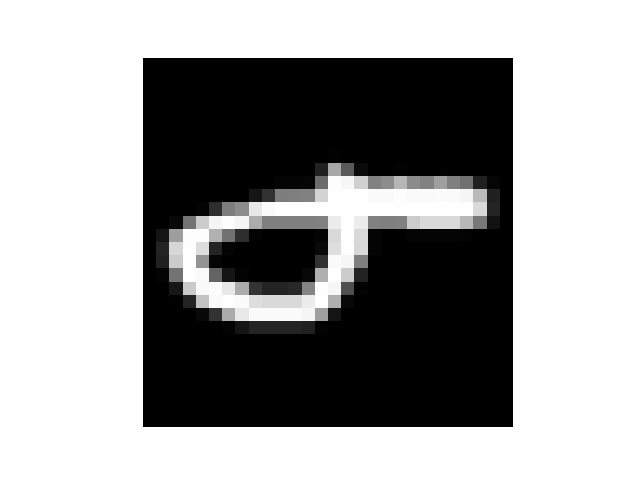
\includegraphics[width=\textwidth]{../res/emnist/sample_1.png}
    \label{fig:emnist_sample_1}
  \end{subfigure}
  \hfill
  \begin{subfigure}[b]{0.3\textwidth}
    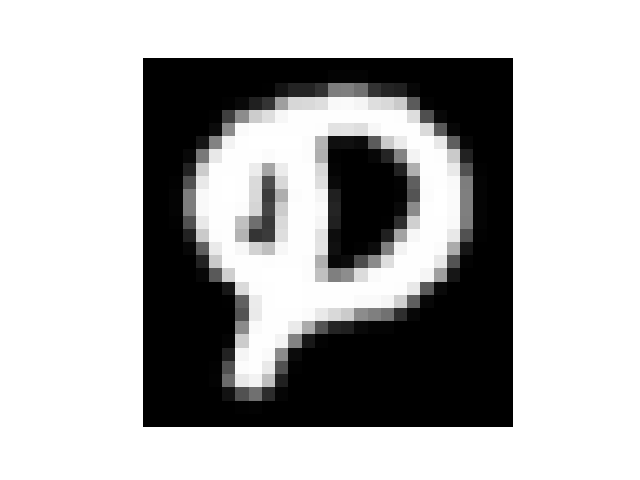
\includegraphics[width=\textwidth]{../res/emnist/sample_2.png}
    \label{fig:emnist_sample_2}
  \end{subfigure}
  \hfill
  \begin{subfigure}[b]{0.3\textwidth}
    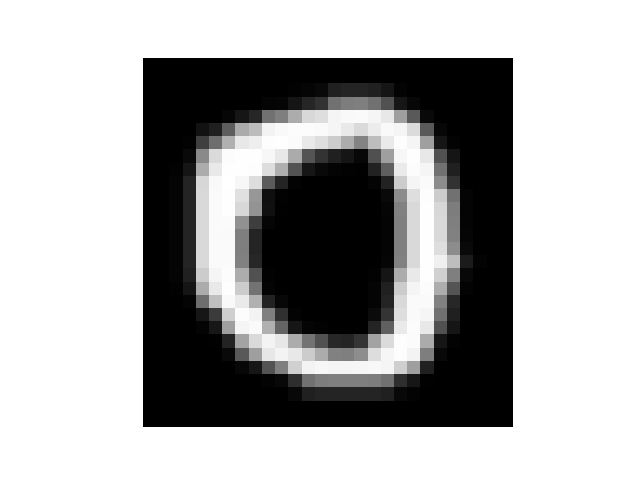
\includegraphics[width=\textwidth]{../res/emnist/sample_3.png}
    \label{fig:emnist_sample_3}
  \end{subfigure}
  \hfill
  \begin{subfigure}[b]{0.3\textwidth}
    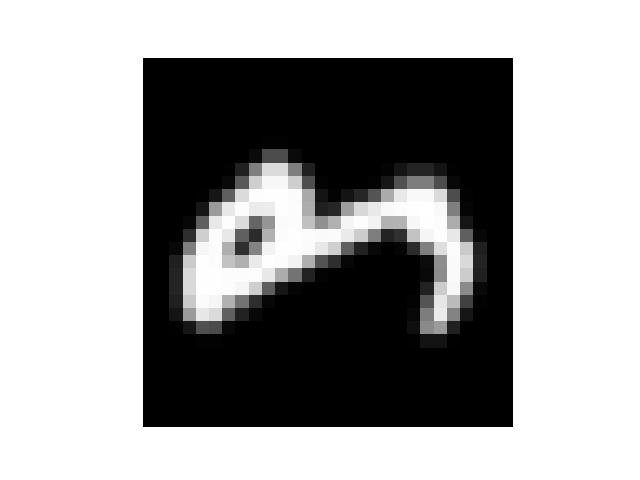
\includegraphics[width=\textwidth]{../res/emnist/sample_4.png}
    \label{fig:emnist_sample_4}
  \end{subfigure}
  \hfill
  \begin{subfigure}[b]{0.3\textwidth}
    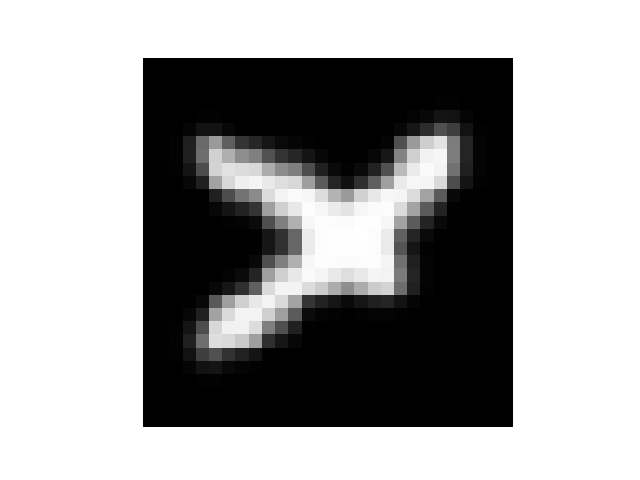
\includegraphics[width=\textwidth]{../res/emnist/sample_5.png}
    \label{fig:emnist_sample_5}
  \end{subfigure}
  \hfill
  \begin{subfigure}[b]{0.3\textwidth}
    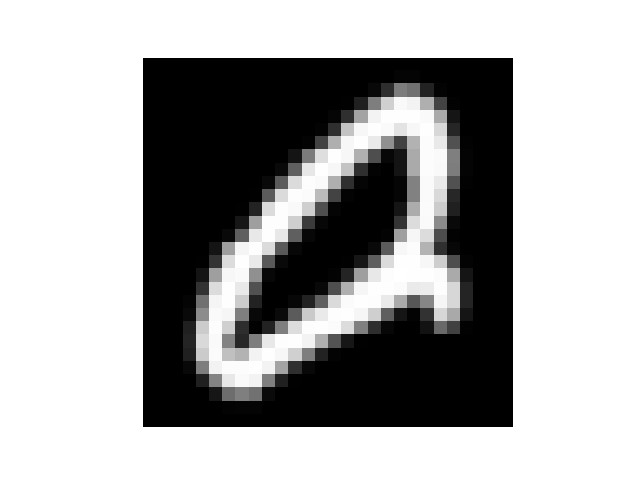
\includegraphics[width=\textwidth]{../res/emnist/sample_6.png}
    \label{fig:emnist_sample_6}
  \end{subfigure}
  \hfill
  \begin{subfigure}[b]{0.3\textwidth}
    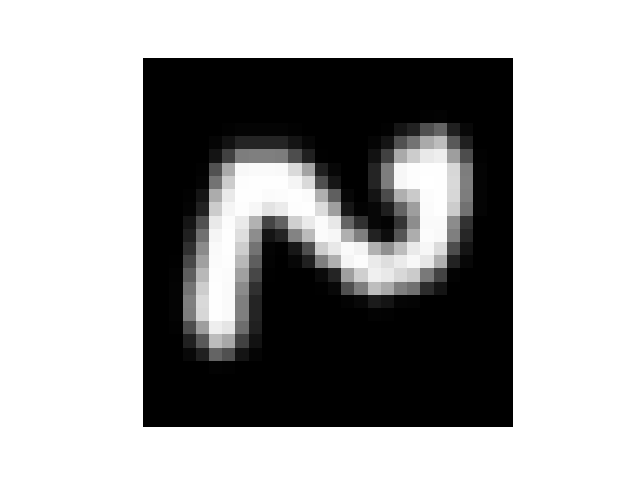
\includegraphics[width=\textwidth]{../res/emnist/sample_7.png}
    \label{fig:emnist_sample_7}
  \end{subfigure}
  \hfill
  \begin{subfigure}[b]{0.3\textwidth}
    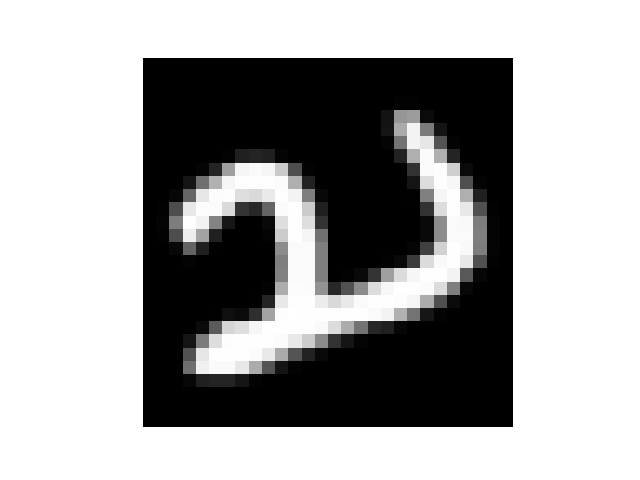
\includegraphics[width=\textwidth]{../res/emnist/sample_8.png}
    \label{fig:emnist_sample_8}
  \end{subfigure}
  
  \caption{Приклади зображень із набора даних \textbf{EMNIST}.}
  \label{fig:emnist_samples}
\end{figure}

\subsection{KMNIST (Kuzushiji MNIST)}
\textbf{KMNIST} --- набір рукописних зображень японських символів з кани (hiragana). Містить 10 класів із по 6000 зображень на кожен клас, також із розміром $28 \times 28$ пікселів у відтінках сірого. Приклади зображень з набору даних можна побачити на рис.\ref{fig:kmnist_samples}. Детальніше про датасет можна дізнатися з офіційного репозиторію \cite{kmnist} та відповідній статті \cite{clanuwat2018deep}.

\begin{figure}[htb]
  \centering

  \begin{subfigure}[b]{0.3\textwidth}
    
\includegraphics[width=\textwidth]{../res/kmnist/sample_0.png}
    \label{fig:kmnist_sample_0}
  \end{subfigure}
  \hfill
  \begin{subfigure}[b]{0.3\textwidth}
    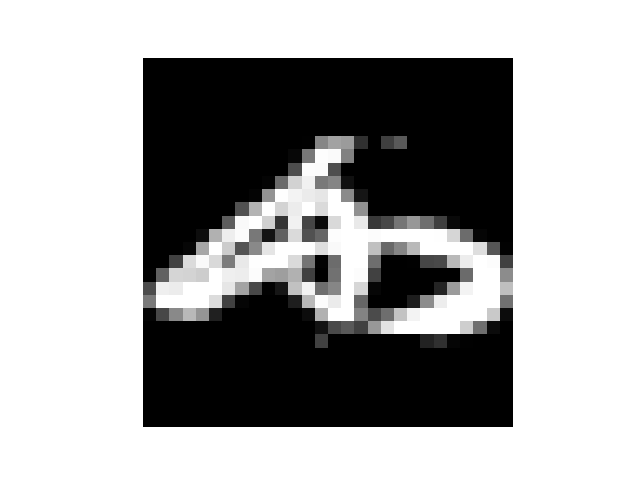
\includegraphics[width=\textwidth]{../res/kmnist/sample_1.png}
    \label{fig:kmnist_sample_1}
  \end{subfigure}
  \hfill
  \begin{subfigure}[b]{0.3\textwidth}
    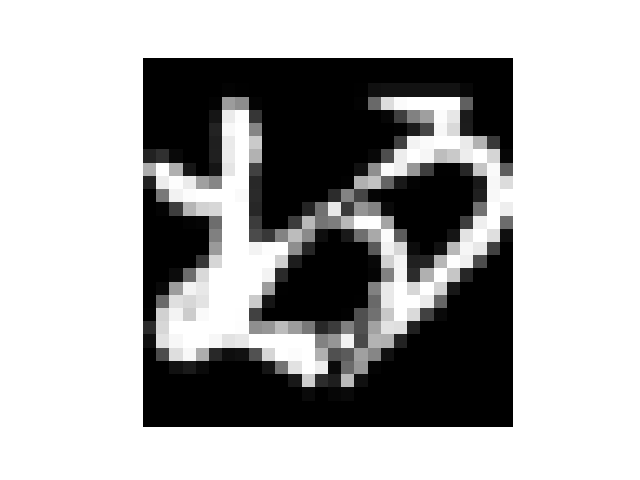
\includegraphics[width=\textwidth]{../res/kmnist/sample_2.png}
    \label{fig:kmnist_sample_2}
  \end{subfigure}
  \hfill
  \begin{subfigure}[b]{0.3\textwidth}
    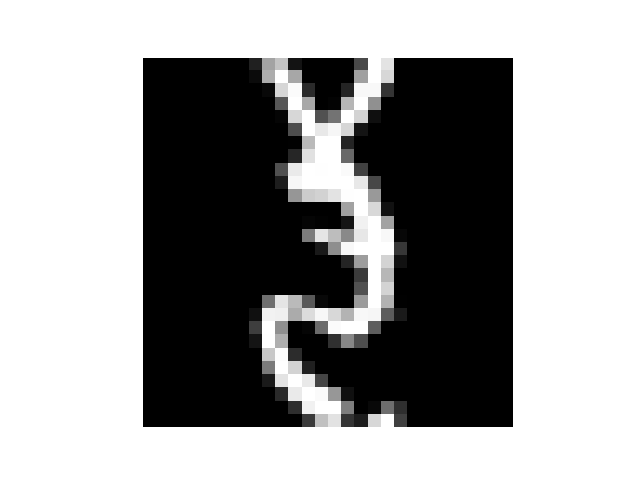
\includegraphics[width=\textwidth]{../res/kmnist/sample_3.png}
    \label{fig:kmnist_sample_3}
  \end{subfigure}
  \hfill
  \begin{subfigure}[b]{0.3\textwidth}
    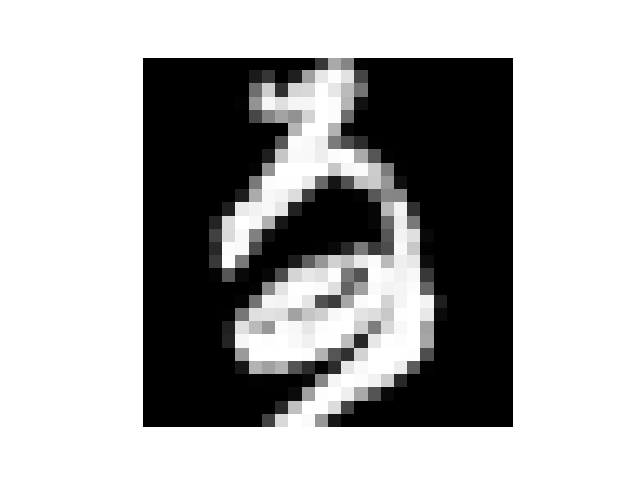
\includegraphics[width=\textwidth]{../res/kmnist/sample_4.png}
    \label{fig:kmnist_sample_4}
  \end{subfigure}
  \hfill
  \begin{subfigure}[b]{0.3\textwidth}
    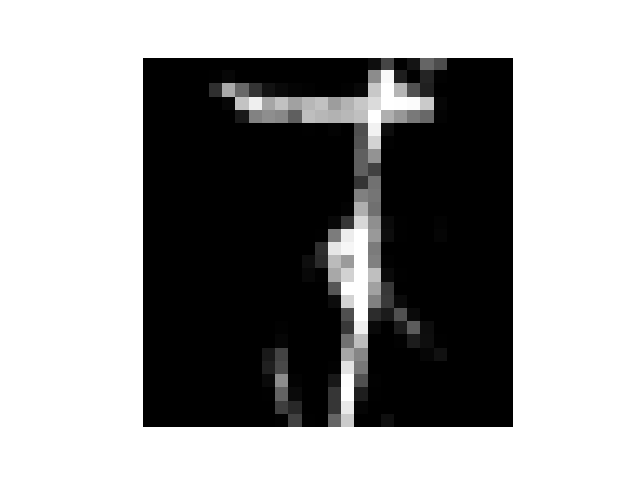
\includegraphics[width=\textwidth]{../res/kmnist/sample_5.png}
    \label{fig:kmnist_sample_5}
  \end{subfigure}
  \hfill
  \begin{subfigure}[b]{0.3\textwidth}
    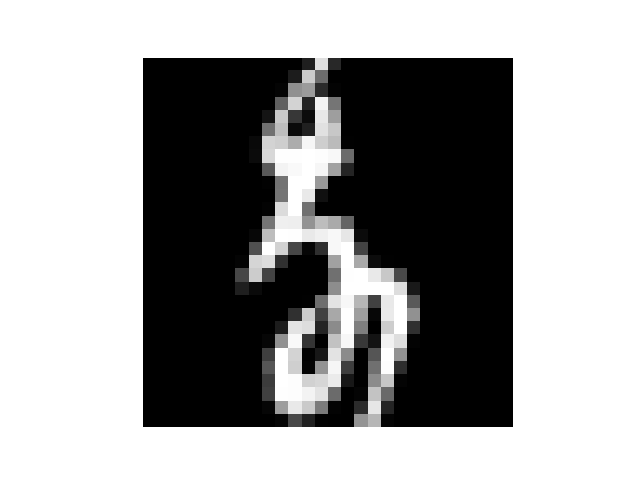
\includegraphics[width=\textwidth]{../res/kmnist/sample_6.png}
    \label{fig:kmnist_sample_6}
  \end{subfigure}
  \hfill
  \begin{subfigure}[b]{0.3\textwidth}
    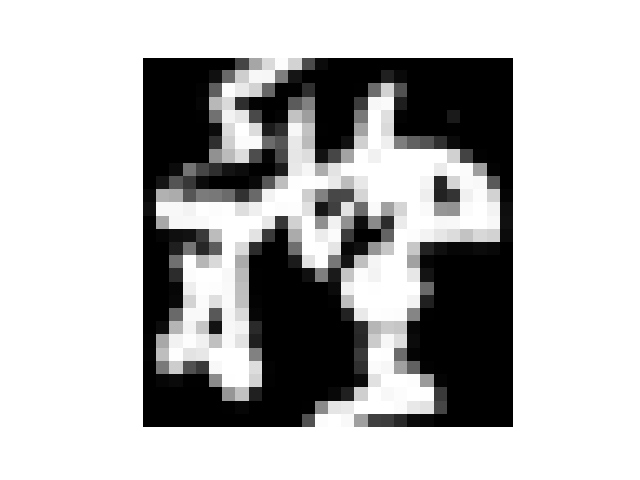
\includegraphics[width=\textwidth]{../res/kmnist/sample_7.png}
    \label{fig:kmnist_sample_7}
  \end{subfigure}
  \hfill
  \begin{subfigure}[b]{0.3\textwidth}
    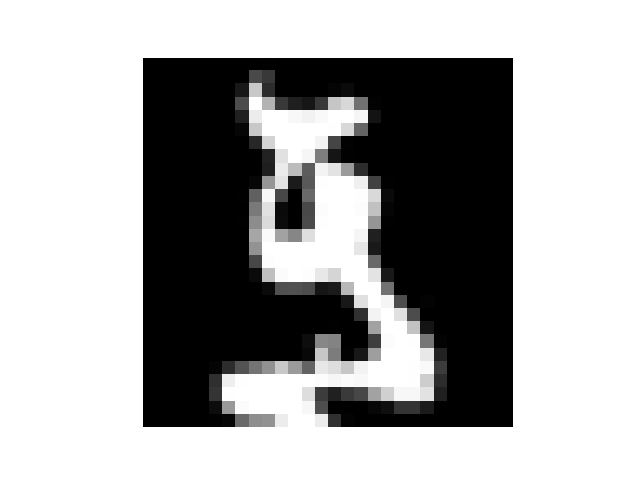
\includegraphics[width=\textwidth]{../res/kmnist/sample_8.png}
    \label{fig:kmnist_sample_8}
  \end{subfigure}
  
  \caption{Приклади зображень із набора даних \textbf{KMNIST}.}
  \label{fig:kmnist_samples}
\end{figure}

\subsection{SVHN (Street View House Numbers)}
\textbf{SVHN} --- кольоровий набір даних, що складається з зображень цифр, виділених із фотографій будинків, зроблених у реальному середовищі. Містить 10 класів (цифри 0–9) з роздільною здатністю $32 \times 32$ пікселі. Приклади зображень з набору даних можна побачити на рис.\ref{fig:svhn_samples}. Набір є більш складним через наявність фону, шуму і різної якості зображень. Офіційний опис доступний за посиланням \cite{svhn}.

\begin{figure}[htb]
  \centering

  \begin{subfigure}[b]{0.3\textwidth}
    
\includegraphics[width=\textwidth]{../res/svhn/sample_0.png}
    \label{fig:svhn_sample_0}
  \end{subfigure}
  \hfill
  \begin{subfigure}[b]{0.3\textwidth}
    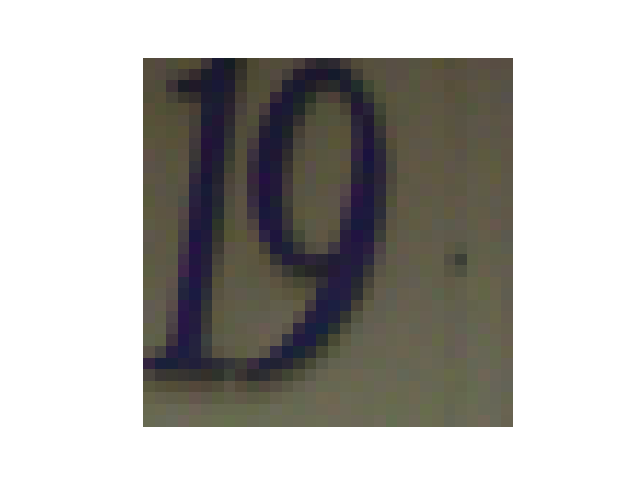
\includegraphics[width=\textwidth]{../res/svhn/sample_1.png}
    \label{fig:svhn_sample_1}
  \end{subfigure}
  \hfill
  \begin{subfigure}[b]{0.3\textwidth}
    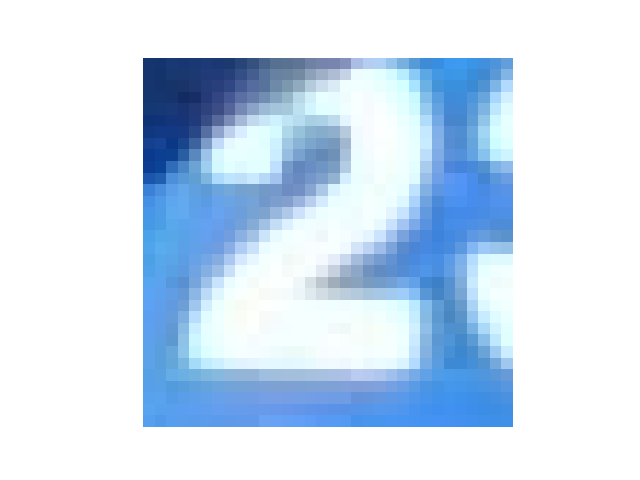
\includegraphics[width=\textwidth]{../res/svhn/sample_2.png}
    \label{fig:svhn_sample_2}
  \end{subfigure}
  \hfill
  \begin{subfigure}[b]{0.3\textwidth}
    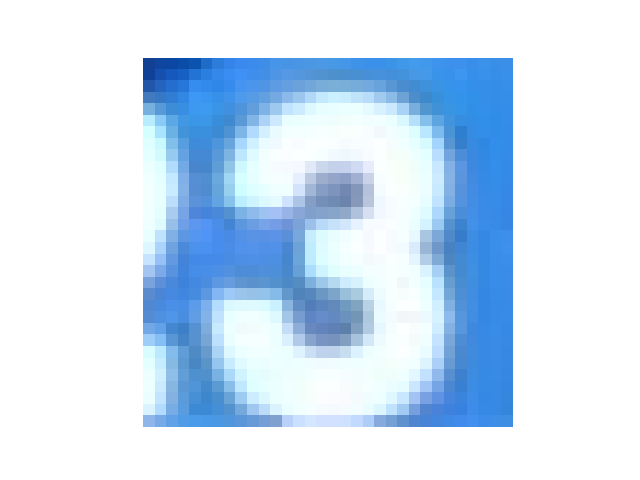
\includegraphics[width=\textwidth]{../res/svhn/sample_3.png}
    \label{fig:svhn_sample_3}
  \end{subfigure}
  \hfill
  \begin{subfigure}[b]{0.3\textwidth}
    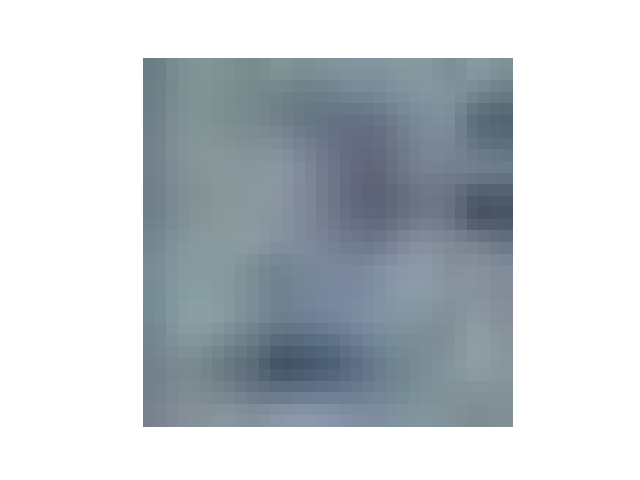
\includegraphics[width=\textwidth]{../res/svhn/sample_4.png}
    \label{fig:svhn_sample_4}
  \end{subfigure}
  \hfill
  \begin{subfigure}[b]{0.3\textwidth}
    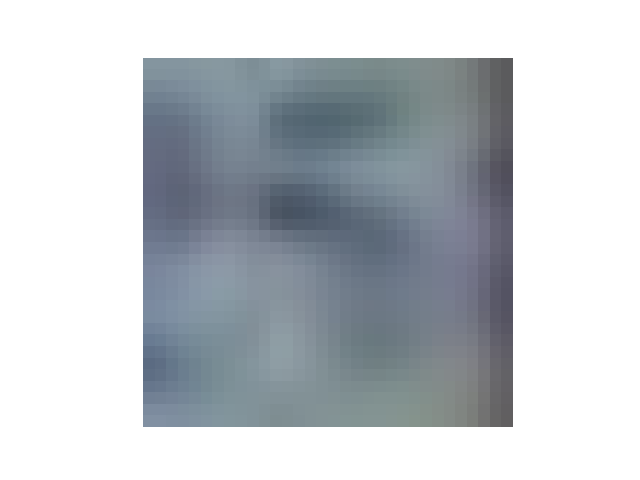
\includegraphics[width=\textwidth]{../res/svhn/sample_5.png}
    \label{fig:svhn_sample_5}
  \end{subfigure}
  \hfill
  \begin{subfigure}[b]{0.3\textwidth}
    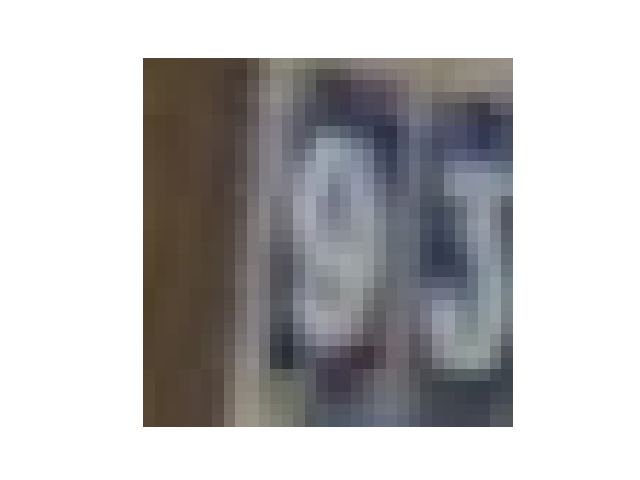
\includegraphics[width=\textwidth]{../res/svhn/sample_6.png}
    \label{fig:svhn_sample_6}
  \end{subfigure}
  \hfill
  \begin{subfigure}[b]{0.3\textwidth}
    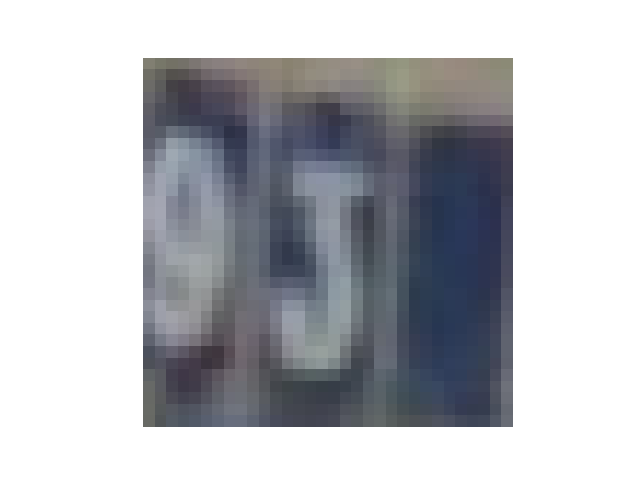
\includegraphics[width=\textwidth]{../res/svhn/sample_7.png}
    \label{fig:svhn_sample_7}
  \end{subfigure}
  \hfill
  \begin{subfigure}[b]{0.3\textwidth}
    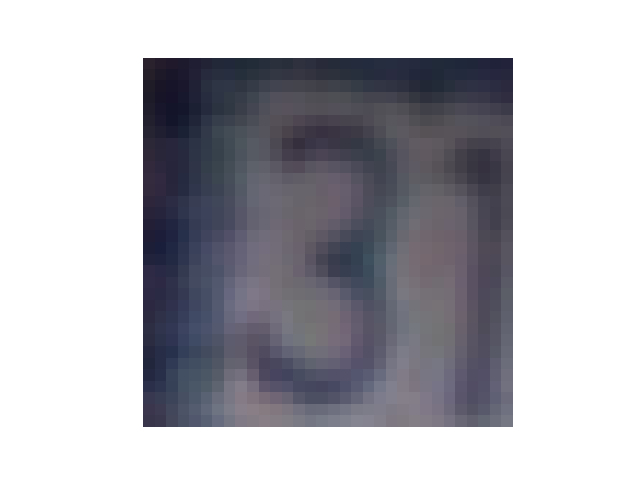
\includegraphics[width=\textwidth]{../res/svhn/sample_8.png}
    \label{fig:svhn_sample_8}
  \end{subfigure}
  
  \caption{Приклади зображень із набора даних \textbf{SVHN}.}
  \label{fig:svhn_samples}
\end{figure}

Різноманітність цих наборів забезпечує комплексну перевірку здатності моделей до узагальнення та адаптації у різних доменах.



\section{Моделі штучних нейронних мереж}
\label{sec:models_}

Для порівняння обрано три сучасні архітектури глибокого навчання, які репрезентують класичні згорткові нейронні мережі (CNN) і новітні трансформерні підходи до обробки зображень.

\subsection{ResNet (Residual Network)}
\textbf{ResNet} --- це архітектура, розроблена для вирішення проблеми затухання градієнту у дуже глибоких нейронних мережах. Вона вводить концепцію \emph{залишкових зв’язків} (skip connections), які додають вихід певного шару до виходу наступного шару, що дає змогу градієнтам ефективно проходити через багато шарів під час зворотного поширення.

У дослідженні застосовано варіант \texttt{ResNet-18}, який має 18 шарів та складається з послідовності залишкових блоків, що складаються із згорткових шарів, нормалізації та функцій активації ReLU. Такий підхід дозволяє моделі мати достатню глибину для виловлювання складних патернів, при цьому не створюючи надмірної обчислювальної складності.

Детальний опис архітектури наведено у статті \cite{resnet}, а офіційна реалізація доступна у документації PyTorch \cite{pytorch_models}.

\subsection{MobileNetV2}
\textbf{MobileNetV2} --- архітектура, розроблена спеціально для мобільних пристроїв і вбудованих систем, де обмежені обчислювальні ресурси та енергоспоживання є критичними.

Основою моделі є \emph{глибинні згортки} (depthwise separable convolutions), які розбивають звичайну згортку на дві операції: окремі згортки по кожному каналу і точкові (pointwise) згортки, що значно зменшує кількість параметрів та обчислень.

Ключовою інновацією MobileNetV2 є \emph{інвертовані залишкові блоки} (inverted residual blocks) з лінійною активацією в кінці блоку, що покращує передачу інформації і зменшує втрати корисної інформації у глибоких шарах.

Детальний опис архітектури наведено в оригінальній роботі \cite{mobilenetv2}, а код та приклади — у документації PyTorch \cite{pytorch_models}.

\subsection{ViT (Vision Transformer)}
\textbf{ViT} --- це модель, яка вперше застосувала трансформерну архітектуру, успішну в обробці природної мови, до завдань комп’ютерного зору.

Модель розбиває вхідне зображення на фіксовані патчі (наприклад, $16 \times 16$ пікселів), кожен з яких перетворюється у вектор-ембеддинг. Ці вектори подаються у трансформер як послідовність токенів, до яких додаються позиційні кодування для збереження просторової інформації.

Самоувага (self-attention) дозволяє моделі враховувати глобальні залежності між різними частинами зображення, що є перевагою у порівнянні зі згортковими мережами, які мають локальний характер обробки.

ViT показав конкурентну точність на великих датасетах і задає новий тренд у комп’ютерному зорі.

Базові принципи описані у статті \cite{vit}, реалізація доступна через репозиторій HuggingFace \cite{huggingface_vit} та сторонні PyTorch-бібліотеки \cite{lucidrains_vit_pytorch}.

\medskip
Усі архітектури використовувалися з попередньо навченими вагами, адаптованими під кількість класів кожного датасету. Навчання та тестування здійснювалися в уніфікованому середовищі з однаковими гіперпараметрами (оптимізатор, learning rate, кількість епох), що дозволяє об'єктивно порівнювати якість та стабільність моделей на різних типах вхідних даних.


\section{Методика тестування}
\label{sec:testing_methodology}

Для об’єктивної оцінки продуктивності моделей у цій роботі застосовано уніфікований підхід до тестування, що забезпечує реплікованість і порівнянність результатів. Код реалізації експериментів, налаштування моделей та скрипти для повторення дослідження доступні на GitHub \cite{neurovisionlab2025}.

\subsection{Попередня обробка даних}
Вхідні зображення нормалізовано до діапазону \([0, 1]\) шляхом поділу піксельних значень на 255. Для кольорового набору SVHN використовувалась перетворення до трьох каналів RGB, тоді як для EMNIST і KMNIST — одиночний канал градацій сірого.

\subsection{Розподіл даних}
Для кожного набору даних використано стандартний поділ на тренувальну, валідаційну та тестову множини, якщо такий передбачений. Якщо валідаційної множини немає, частина тренувальних даних (10–15\%) виділялася для валідації.

\subsection{Параметри навчання}
Всі моделі навчалися із застосуванням однакових гіперпараметрів: 

\begin{itemize}[leftmargin=*]
  \item Оптимізатор: Adam із початковою швидкістю навчання \(10^{-3}\),
  \item Розмір батчу: 64,
  \item Кількість епох: 15,
  \item Регуляризація: відсутня (для чистоти порівняння),
  \item Функція втрат: категоріальна крос-ентропія.
\end{itemize}

\subsection{Оцінка якості моделей}
Для вимірювання точності класифікації застосовано метрику \textbf{accuracy} — відношення правильно класифікованих прикладів до загальної кількості в тестовому наборі.

Окрім accuracy, для більш глибокого аналізу якості класифікації розраховували такі метрики як \textbf{Precision} (точність), \textbf{Recall} (повнота) та \textbf{F1-score} — гармонійне середнє між точністю і повнотою. Ці показники дозволяють оцінити баланс між правильними позитивними прогнозами та пропущеними випадками, що особливо важливо при роботі з дисбалансованими класами.

Додатково проаналізовано динаміку збіжності на тренувальній та валідаційній множинах для оцінки стійкості та уникнення перенавчання, а також матрицю плутанини. Було проведено оцінку розміру моделі та обсягу використаної \textbf{VRAM} (відеопам'яті) під час навчання і тестування для визначення ресурсних вимог кожної архітектури.

\subsection{Апаратура та програмне забезпечення}
Експерименти виконувалися на робочій станції з GPU NVIDIA RTX 4070 SUPER. Використовувались бібліотеки PyTorch (версія 2.7.0) та стандартні інструменти для обробки даних та візуалізації результатів.



\section{Результати експериментів}  
\label{sec:results}

У результаті проведених експериментів було отримано кількісні показники продуктивності трьох архітектур на тестових наборах даних. Нижче наведені результати для трьох датасетів: SVHN, EMNIST та KMNIST. Для кожного датасету наведено основні метрики класифікації: accuracy, F1-міра, precision і recall (Табл.\ref{tab:metrics_all}).

\begin{table}[h!]
\centering
\caption{Порівняння продуктивності моделей на різних датасетах}
\label{tab:metrics_all}
\begin{tabular}{llcccc}
\toprule
Датасет & Модель & Accuracy & F1-міра & Precision & Recall \\
\midrule
\multirow{3}{*}{EMNIST} 
  & ResNet & 94.71\% & 94.69\% & 94.82\% & 94.71\% \\
  & MobileNet & 95.03\% & 95.03\% & 95.09\% & 95.03\% \\
  & ViT & 88.89\% & 88.87\% & 89.46\% & 88.89\% \\
\midrule
\multirow{3}{*}{KMNIST}
  & ResNet & 97.24\% & 97.23\% & 97.26\% & 97.24\% \\
  & MobileNet & 97.79\% & 97.79\% & 97.82\% & 97.79\% \\
  & ViT & 90.58\% & 90.58\% & 90.71\% & 90.58\% \\
\midrule
\multirow{3}{*}{SVHN}
  & ResNet & 94.29\% & 94.30\% & 94.46\% & 94.29\% \\
  & MobileNet & 95.79\% & 95.79\% & 95.82\% & 95.79\% \\
  & ViT & 89.7\% & 89.6\% & 89.6\% & 89.7\% \\
\bottomrule
\end{tabular}
\end{table}

Окрім якісних характеристик, було проаналізовано час навчання та максимальні обсяги використаної VRAM під час навчання ($\tau$) та класифікації на тренувальному наборі даних (Табл.\ref{tab:resources}).

\begin{table}[h!]
\centering
\caption{Ресурсні характеристики моделей}
\label{tab:resources}
\begin{tabular}{llcccc}
\toprule 
Датасет & Модель & $\tau$ (c) & Train VRAM (MB) & Test VRAM (MB) \\
\midrule
\multirow{3}{*}{EMNIST} 
  & ResNet & 2523 & 876.80 & 423.50 \\
  & MobileNet & 4689 & 2466.56 & 310.02 \\
  & ViT & 18157 & 4945.70 & 1600.37 \\
\midrule
\multirow{3}{*}{KMNIST}
  & ResNet & 1360 & 1268.81 & 815.51 \\
  & MobileNet & 2350 & 2858.38 & 601.84 \\
  & ViT & 8881 & 5337.65 & 1992.32 \\
\midrule
\multirow{3}{*}{SVHN}
  & ResNet & 1693 & 1281.14 & 827.86 \\
  & MobileNet & 2892 & 2870.64 & 614.10 \\
  & ViT & 11196 & 5354.40 & 2010.57 \\
\bottomrule
\end{tabular}
\end{table}


\section{Порівняльний аналіз}
\label{sec:analysis}

У цьому розділі проведено порівняльний аналіз трьох архітектур нейронних мереж (ResNet, MobileNet та ViT) на основі результатів експериментів, наведених у розділі \ref{sec:results}. Аналіз охоплює як якісні характеристики точності класифікації, так і ресурсні вимоги кожної моделі.

\subsection{Аналіз точності класифікації}

Аналізуючи метрики якості класифікації з таблиці \ref{tab:metrics_all}, можна зробити такі висновки:

MobileNet демонструє найвищу точність класифікації на всіх трьох датасетах (95.03\% на EMNIST, 97.79\% на KMNIST та 95.79\% на SVHN), випереджаючи ResNet на 0.3–1.5 процентних пункти. Архітектура ViT суттєво поступається згортковим моделям із різницею в точності від 4.6\% до 7.2\%.

Виникає здивування, що Vision Transformer демонструє суттєво гірші результати порівняно зі згортковими мережами. Та це можна пояснити кількома ключовими факторами:

По-перше, ViT потребує значно більших обсягів тренувальних даних для ефективного навчання. Ця модель спроєктована для роботи з великими наборами даних, такими як ImageNet-21k \cite{imagenet21k} або JFT-300M \cite{googlejft300m, mahajan2018exploring}, де вона має змогу навчитися складних патернів завдяки численним прикладам \cite{dosovitskiy2020vit}. У задачах із обмеженою кількістю зразків, як у нашому випадку, ViT часто піддається перенавчанню або не здатна знайти оптимальні представлення.

По-друге, трансформери не мають вбудованих індуктивних обмежень, характерних для згорткових мереж, таких як локальна зв’язність і просторові ієрархії. Ці індуктивні обмеження дозволяють згортковим мережам ефективно виявляти важливі ознаки навіть на невеликих датасетах, тоді як ViT повинна навчатися цих властивостей з нуля, що вимагає більше даних і часу \cite{convit2021, bridginggap2022}.

% По-третє, механізм self-attention у ViT має високу обчислювальну складність і потребує значних ресурсів пам’яті, що ускладнює її застосування на обмежених за потужністю системах і ускладнює оптимізацію під час тренування.
% Нарешті, ефективність ViT значно зростає при попередньому навчанні на великих наборах даних з подальшою тонкою настройкою, що не було реалізовано в рамках наших експериментів.

Отже, незважаючи на потенціал трансформерних архітектур, у задачах із відносно невеликими датасетами згорткові мережі (MobileNet та ResNet) залишаються більш ефективними та ресурсозберігаючими рішеннями.

Для всіх моделей спостерігається висока узгодженість між різними метриками (Accuracy, F1-міра, Precision, Recall), що свідчить про збалансовану класифікацію без суттєвого зміщення на користь окремих класів.

\subsection{Аналіз ресурсних вимог}

Розглядаючи дані таблиці \ref{tab:resources}, можна виділити такі ключові моменти:

Архітектура ResNet навчається найшвидше на всіх датасетах — приблизно в 1.7–1.9 раза швидше за MobileNet та в 6.5–7.2 раза швидше за ViT. Повільне навчання ViT є суттєвим недоліком при обмежених обчислювальних ресурсах. Це пов’язано з тим, що механізм self-attention у ViT має високу обчислювальну складність — з квадратичною залежністю від розміру вхідного зображення — і потребує значних ресурсів пам’яті. Така особливість ускладнює застосування ViT на обмежених за потужністю системах і робить оптимізацію моделі під час тренування більш складною \cite{vaswani2017attention, dosovitskiy2020vit}.

ViT споживає найбільше відеопам’яті під час тренування (4.9–5.4 ГБ), що в 1.8–2 раза більше, ніж MobileNet, і в 4.1–5.6 раза більше, ніж ResNet. Найекономнішим у цьому плані є ResNet. При інференсі зберігається дещо інша тенденція: ViT вимагає найбільше ресурсів, MobileNet — найменше, а ResNet коливається від помірного до середнього використання. ResNet споживає менше пам’яті та навчається швидше, ніж MobileNet, хоча має більше параметрів. Водночас MobileNet під час тренування використовує більше пам’яті і часу, але на інференсі (тестовому проході) є найбільш економною моделлю. Це пояснюється архітектурними особливостями та особливостями реалізації:

MobileNet застосовує depthwise separable convolutions, які значно зменшують кількість параметрів і обчислень у порівнянні зі стандартними згортками. Проте ця техніка призводить до більшої кількості дрібних операцій, що створює додаткові накладні витрати на обробку та менш ефективне використання апаратних прискорювачів під час тренування \cite{howard2017mobilenets, sandler2018mobilenetv2}.

ResNet використовує класичні згортки та залишкові зв’язки (residual connections), які допомагають стабілізувати і пришвидшити процес навчання, полегшуючи проходження градієнтів. Крім того, згорткові операції у ResNet добре оптимізовані в апаратних бібліотеках (наприклад, cuDNN), що забезпечує ефективніше використання пам’яті і швидшу обробку \cite{he2016deep, szegedy2017inception}.

Під час інференсу MobileNet споживає менше ресурсів завдяки меншій кількості параметрів і обчислень, що робить його більш економним у порівнянні з ResNet \cite{howard2017mobilenets, sandler2018mobilenetv2}. 

Тобто, велика кількість дрібних операцій у MobileNet збільшує накладні витрати під час тренування, тоді як ResNet виграє у швидкості й ефективності навчання через оптимізації архітектури та апаратної підтримки.



\section{Висновки}
\label{sec:conclusions}
Базуючись на проведеному вище аналізі, можна зробити наступні висновки:

Для розгортання на продуктивних системах з обмеженими ресурсами (особливо на мобільних пристроях) оптимальним є використання MobileNet, яка забезпечує найвищу точність при помірних вимогах до пам'яті під час інференсу.

Для швидкого прототипування або навчання на обмежених обчислювальних ресурсах доцільно використовувати ResNet, яка демонструє найшвидше навчання та добрий баланс між швидкістю та точністю класифікації.

Використання архітектури ViT без додаткових оптимізацій, великого обсягу даних або модифікацій не рекомендується через суттєво вищі вимоги до ресурсів та тривалість навчання. Загалом, для задач класифікації зображень на відносно невеликих датасетах згорткові мережі (MobileNet і ResNet) показують кращий баланс між точністю та обчислювальними витратами, ніж трансформерні моделі.



\newpage
\printbibliography[heading=bibintoc,title={Список використаних джерел}]

\end{document}